\subsection{Generalized Surface inFiltration Baseflow model (model ID: 20)}
The GSFB model (fig.~\ref{fig:20_schematic}) is  originally developed for use in Australian ephemeral catchments \citep{Nathan1990,Ye1997}. It has 3 stores and 8 parameters ($C$, $NDC$, $S_{max}$, $E_{max}$, $F_{rate}$, $B$, $DPF$ and $SDR_{max}$). The model aims to represent:

\begin{itemizecompact}
\item Saturation excess surface runoff;
\item Threshold-based infiltration;
\item Threshold-based baseflow;
\item Deep percolation and water rise to meet evaporation demand.
\end{itemizecompact}

\subsubsection{File names}
\begin{tabular}{@{}ll}
Model: &m\_20\_gsfb\_8p\_3s \\
Parameter ranges: &m\_20\_gsfb\_8p\_3s\_parameter\_ ranges \\
\end{tabular}

% Equations
\subsubsection{Model equations}

% Model layout figure
{ 																	% This ensures it doesn't warp text further down
\begin{wrapfigure}{l}{4.5cm}
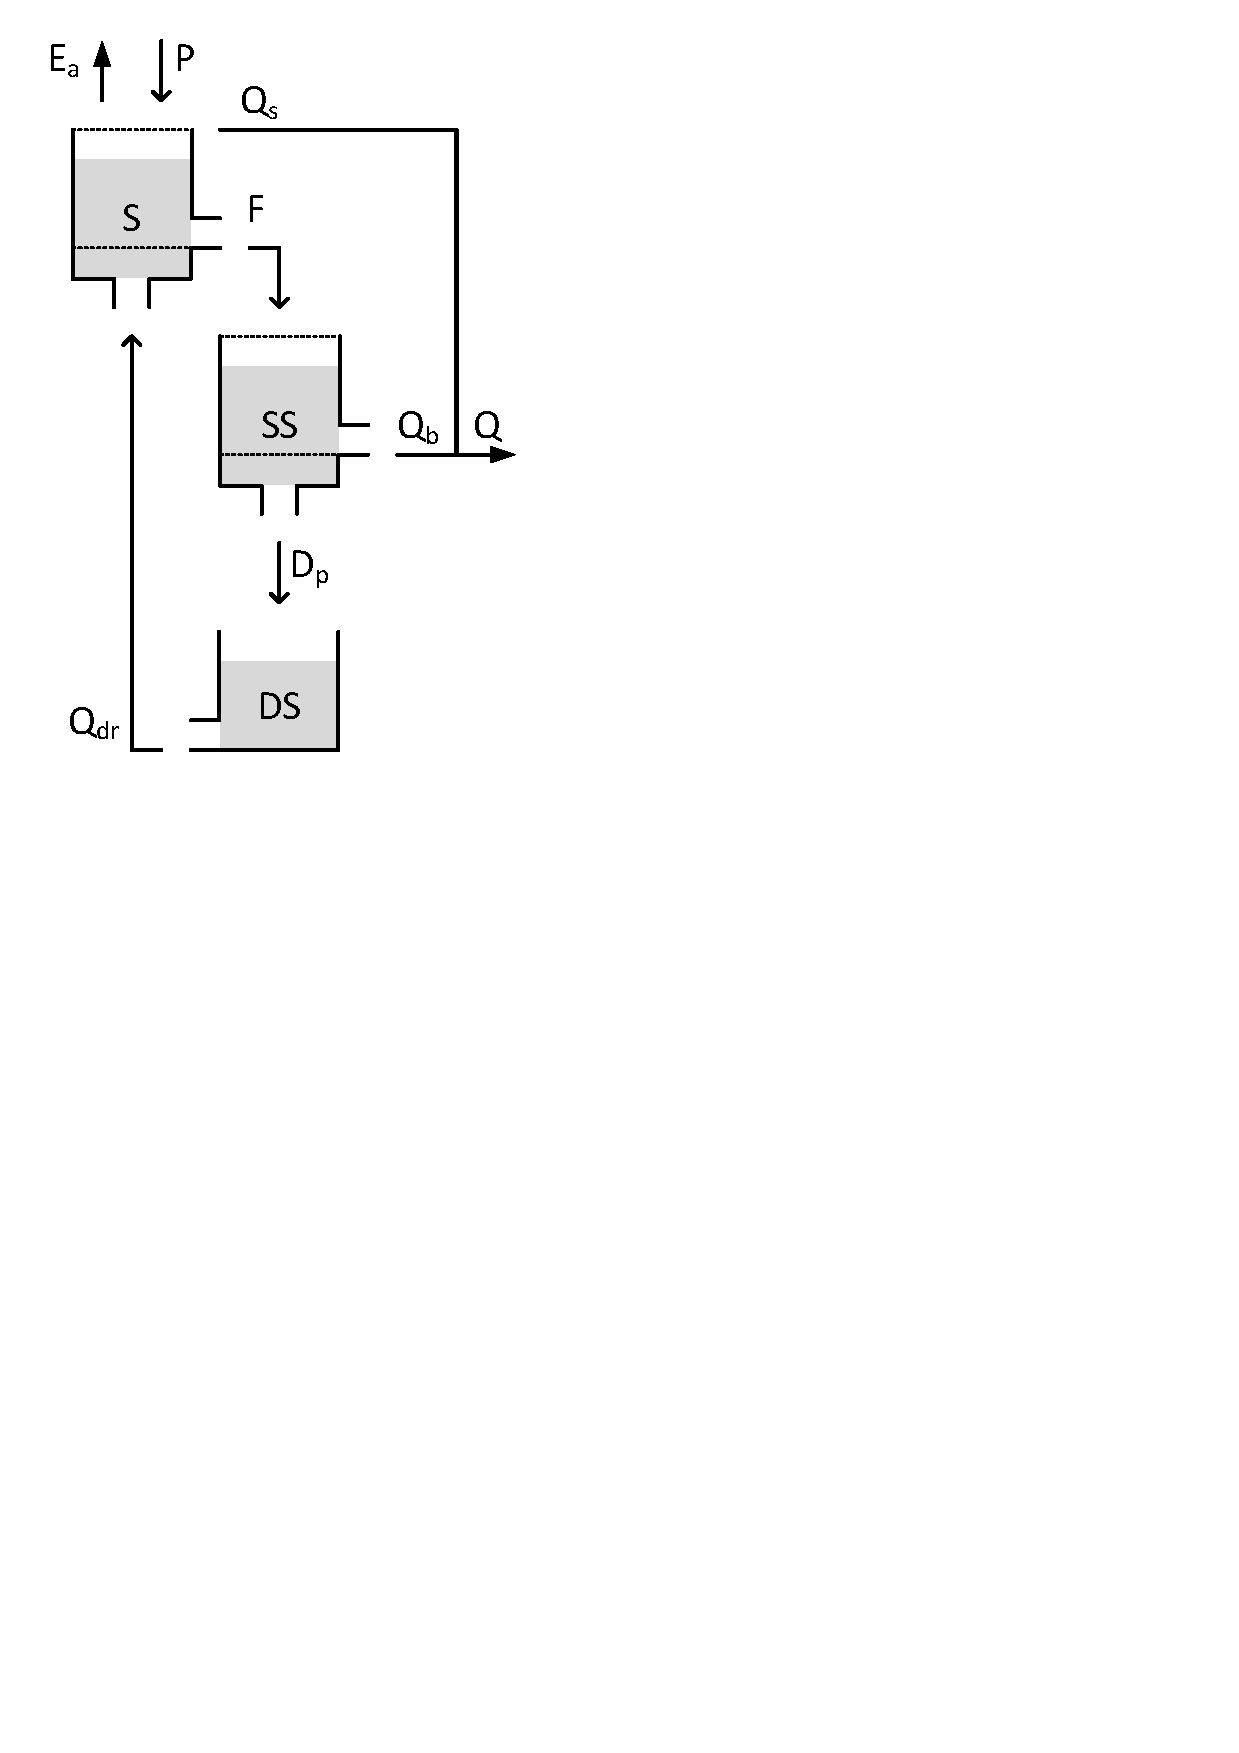
\includegraphics[trim=1cm 17cm 7cm 1cm,width=7cm,keepaspectratio]{./files/20_schematic.pdf}
\caption{Structure of the GSFB model} \label{fig:20_schematic}
\end{wrapfigure}

\begin{align}
	\frac{dS}{dt} &= P + Q_{dr}- E_a -Q_s-F \\
	Q_{dr} &= \begin{cases}
		C*DS*\left(1-\frac{S}{NDC*S_{max}}\right), &\text{if } S \leq NDC*S_{max} \\
		0, & \text{otherwise} \\
	\end{cases} \\
	E_a &= 
	\begin{cases}
		E_p, & \text{if } S > NDC*S_{max} \\
		min\left(E_p, E_{max}\frac{S}{NDC*S_{max}}\right), & \text{otherwise}
	\end{cases} \\
	Q_s &= \begin{cases}
		P, &\text{if } S = S_{max} \\
		0, & \text{otherwise} \\
	\end{cases} \\
	F &= \begin{cases}
		F_{rate}, &\text{if } S > NDC*S_{max} \\
		0, & \text{otherwise} \\
	\end{cases} 
\end{align}

} % end of wrapfigure fix
\vspace{1cm}

Where $S$ [mm] is the current storage in the upper zone, refilled by precipitation $P$ $[mm/d]$ and recharge from deep groundwater $Q_{dr}$ $[mm/d]$. 
The store is drained by evaporation $E_a$ $[mm/d]$, surface runoff $Q_{s}$ $[mm/d]$ and infiltration $F$ $[mm/d]$.
$E_a$ occurs at the potential rate $E_p$ $[mm/d]$ if the store is above a threshold capacity given as the fraction $NDC$ [-] of maximum storage $S_{max}$ [mm].
Evaporation occurs at a reduced rate scaled by maximum evaporation rate $E_{max}$ $[mm/d]$ if the store is below this threshold.
$Q_s$ occurs only if the store is at maximum capacity $S_{max}$. 
$F$ occurs at a constant rate $F_{rate}$ if the store is above threshold $NDC*S_{max}$.
Recharge from deep percolation only occurs if the store is below threshold capacity $NDC*S_{max}$ and uses time parameter $C$ $[d^{-1}]$ and current deep storage $DS$ [mm].

\begin{align}
	\frac{dSS}{dt} &=F - Q_b-D_p\\
	Q_b &= \begin{cases}
		B*DPF*(SS-SDR_{max}), &\text{if } SS > SDR_{max} \\
		0, & \text{otherwise} \\
	\end{cases} \\
	D_p &= (1-B)*DPF*SS
\end{align}

Where $SS$ [mm] is the current storage in the subsurface store, refilled by infiltration $F$ and drained by baseflow $Q_b$ $[mm/d]$ and deep percolation $D_p$ $[mm/d]$.
Outflow from this store is given as a function of storage $DS$ and time coefficient  $DPF$ $[d^{-1}]$.
A fraction $1-B$ [-] of this outflow is deep percolation $D_p$.
The remaining fraction $B$ [-] is baseflow $Q_b$, provided the store is above threshold $SDR_{max}$ [mm].

\begin{align}
	\frac{dDS}{dt} &= D_p - Q_{dr}  \\
\end{align}
  
Where $DS$ [mm] is the current storage in the deep store, refilled by a deep percolation $D_p$ and drained by recharge to the upper store $Q_{dr}$.
Total flow:

\begin{align}
	Q_t &= Q_s+Q_b
\end{align}

\subsubsection{Parameter overview}

% Table generated by Excel2LaTeX from sheet 'Sheet1'
\begin{table}[htbp]
  \centering
    \begin{tabular}{lll}
    \toprule
    Parameter & Unit  & Description \\
    \midrule
    $C$   & $d^{-1}$ & Recharge coefficient \\
    $NDC$ & $-$   & Threshold for evaporation and recharge as fraction of $S_{max}$ \\
    $S_{max}$ & $mm$  & Maximum soil moisture storage \\
    $E_{max}$ & $mm~d^{-1}$ & Maximum evaporation rate \\
    $F_{rate}$ & $mm~d^{-1}$ & Recharge rate \\
    $B$   & $-$   & Fraction subsurface flow to stream \\
    $DPF$ & $d^{-1}$ & Runoff coefficient \\
    $SDR_{max}$ & $mm$  & Threshold for subsurface flow generation \\
    \bottomrule
    \end{tabular}%
  \label{tab:addlabel}%
\end{table}%
